
\documentclass{beamer}
\usecolortheme{dove}
\setbeamertemplate{navigation symbols}{}
\setbeamertemplate{footline}[text line]{\parbox{\linewidth}{\vspace*{-8pt}\insertsectionnavigationhorizontal{.95\paperwidth}{\hspace{-32pt}}{\hfill\hfill}}}
\usepackage{amsmath,amssymb,amsfonts,amsthm, multicol, subfigure, color}
\usepackage{bm}
\usepackage{graphicx}
\usepackage{tabularx}
\usepackage{booktabs}
\usepackage{hyperref}
\usepackage{pdfpages}
\usepackage{xcolor}
\definecolor{seagreen}{RGB}{46, 139, 87}
\definecolor{ucla}{RGB}{39, 116, 174}
\definecolor{darkestblue}{RGB}{0, 59, 92}
\definecolor{gold}{RGB}{255, 209, 0}
\def\independenT#1#2{\mathrel{\rlap{$#1#2$}\mkern2mu{#1#2}}}
\newcommand\indep{\protect\mathpalette{\protect\independenT}{\perp}}
\def\log{\text{log}}
\newcommand\logit{\text{logit}}
\newcommand\iid{\stackrel{\text{iid}}{\sim}}
\newcommand\E{\text{E}}
\newcommand\V{\text{V}}
\renewcommand\P{\text{P}}
\newcommand{\Cov}{\text{Cov}}
\newcommand{\Cor}{\text{Cor}}
\newcommand\doop{\text{do}}
\usepackage{stackrel}
\usepackage{tikz}
\usetikzlibrary{arrows,shapes.arrows,positioning,shapes,patterns,calc}
\newcommand\slideref[1]{\vskip .1cm \tiny \textcolor{gray}{{#1}}}
\newcommand\red[1]{\color{red}#1}
\newcommand\blue[1]{\color{blue}#1}
\newcommand\gray[1]{\color{gray}#1}
\newcommand\seagreen[1]{\color{seagreen}#1}
\newcommand\purple[1]{\color{purple}#1}
\newcommand\orange[1]{\color{orange}#1}
\newcommand\black[1]{\color{black}#1}
\newcommand\white[1]{\color{white}#1}
\newcommand\teal[1]{\color{teal}#1}
\newcommand\magenta[1]{\color{magenta}#1}
\newcommand\Fuchsia[1]{\color{Fuchsia}#1}
\newcommand\BlueGreen[1]{\color{BlueGreen}#1}
\newcommand\bblue[1]{\textcolor{blue}{\textbf{#1}}}
\newcommand\bred[1]{\textcolor{red}{\textbf{#1}}}
\newcommand\bgray[1]{\textcolor{gray}{\textbf{#1}}}
\newcommand\bgreen[1]{\textcolor{seagreen}{\textbf{#1}}}
\newcommand\bref[2]{\href{#1}{\color{blue}{#2}}}
\colorlet{lightgray}{gray!40}
\pgfdeclarelayer{bg}    % declare background layer for tikz
\pgfsetlayers{bg,main} % order layers for tikz
\newcommand\mycite[1]{\begin{scriptsize}\textcolor{darkgray}{(#1)}\end{scriptsize}}
\newcommand{\tcframe}{\frame{
%\small{
\only<1|handout:0>{\tableofcontents}
\only<2|handout:1>{\tableofcontents[currentsubsection]}}
%}
}
\usepackage{soul}

\usepackage[round]{natbib}
\bibliographystyle{humannat-mod}
\setbeamertemplate{enumerate items}[default]
\usepackage{mathtools}

\newcommand{\goalsframe}{\begin{frame}{Learning goals for today}
By the end of class, you will be able to use an \textbf{outcome model} in the service of
\begin{itemize}
    \item describing a population from a non-probability sample
    \item inferring average causal effects in an observational study
\end{itemize} \vskip .2in
\end{frame}}

\title{Estimation by Prediction}
\author{UCLA SOCIOL 212B\\Winter 2025}
\date{26 Feb 2025}

\begin{document}

\maketitle

\goalsframe

\section{Prediction For Population Inference}

\begin{frame}
\huge Predicting outcomes for population inference from non-probability samples
\end{frame}

\begin{frame}

Survey on Amazon Mechanical Turk

\begin{enumerate}
\item What is your sex?
\item What is your age?
\item Have you ever had a TikTok account?
\end{enumerate}

Why might the sample mean of $Y$ be a poor estimator of the mean in the full U.S. population?

\end{frame}

\begin{frame}{A possible (but heroic) assumption}

Conditionally exchangeable sampling:
$$
\underbrace{S}_{\text{Sampling}} \indep \underbrace{Y}_{\text{Ever had TikTok}} \mid \underbrace{\vec{X}}_{\text{Sex, Age}}
$$
Equivalently: ${\text{P}}(Y\mid S = 1, \vec{X} = \vec{x}) = {\text{P}}(Y \mid \vec{X} = \vec{x})$
 \vskip .1in
Then sample data on 52-year-old men is informative about the population mean among 52-year-old men \pause
\vskip .2in
\textbf{Problems:}
\begin{itemize}
\item Many age $\times$ sex subgroups! Small sample.
\item How to aggregate the subgroup estimates?
\end{itemize}

\end{frame}

\begin{frame}{Step 1: Model the conditional probabilities}

$$\text{logit}\left(\hat{\text{P}}(Y = 1\mid S = 1, \vec{X})\right) = \hat\beta_0 + \hat\beta_1(\text{Sex = Female}) + \hat\beta_2 (\text{Age})$$ \

\end{frame}

\begin{frame}{Step 2: Define $\vec{X}$ distribution to aggregate}

U.S. Census has estimates of the age $\times$ sex distribution:\\$\P(\vec{X} = \vec{x})$ is known

\end{frame}

\begin{frame}{Overall strategy}

$$
\hat{\text{P}}(Y) = \sum_{\vec{x}}\hat{\text{P}}(Y\mid\vec{X} = \vec{x}){\text{P}}(\vec{X} = \vec{x})
$$

\begin{itemize}
\item measure $\vec{X}$ and $Y$ in a non-probability sample
\item measure $\vec{X}$ in a probability sample or census
\item assume exchangeable sampling given $\vec{X}$ (heroic!)
\item model $\text{E}(Y\mid\vec{X})$ or $\text{P}(Y\mid\vec{X})$ in the non-probability sample
\item estimate $\text{P}(\vec{X} = \vec{x})$ in the probability sample or census
\item re-aggregate $\hat{\text{E}}(Y\mid\vec{X})$ using the weights $\hat{\text{P}}(\vec{X} = \vec{x})$ 
\end{itemize}

\end{frame}

\begin{frame}{Real example: Xbox survey}{\bref{https://doi.org/10.1016/j.ijforecast.2014.06.001}{Wang et al. 2015}}

Survey in 2012:\\
If the election were held today, who would you vote for?\\(Obama or Romney) \vskip .2in \pause
Survey conducted on Xbox. Disproportionately young men. \\ \pause
But over 700,000 responses!

\end{frame}

\begin{frame}{Real example: Xbox survey}{\bref{https://doi.org/10.1016/j.ijforecast.2014.06.001}{Wang et al. 2015}}

Measured $\vec{X}$ in hopes of conditional exchangeability: \\
sex, race, age, education, state, party ID, political ideology, and who they voted for in the 2008 presidential election. \vskip .2in
Hope for: $Y\indep S \mid \vec{X}$

\end{frame}

\begin{frame}{Real example: Xbox survey}{\bref{https://doi.org/10.1016/j.ijforecast.2014.06.001}{Wang et al. 2015}}

Step 1: Estimate conditional means
$$
\hat{\text{P}}(Y = 1\mid S = 1,\vec{X} = \vec{x}) = \text{logit}^{-1}(\text{complicated function of }\vec{x})
$$

Step 2: Estimate $\P(\vec{X} = \vec{x})$ using 2008 exit polls \vskip .1in

Step 3: Aggregate predictions from (1) weighted by (2):

$$
\hat{\text{P}}(Y = 1) = \sum_{\vec{x}}\underbrace{\hat{\text{P}}(\vec{X} = \vec{x})}_{\substack{\text{Stratum size,}\\\text{estimated from}\\\text{2008 exit polls}}}\underbrace{\hat{\text{P}}(Y = 1\mid S = 1,\vec{X} = \vec{x})}_{\substack{\text{Prediction within the stratum,}\\\text{estimated from Xbox survey}}}
$$ \pause

\textbf{They did surprisingly well!}

\end{frame}

\begin{frame}{Takeaways: Prediction to describe}


predictive outcome models $\hat{f}:\vec{X}\rightarrow \hat{Y}$\\learned in non-probability samples

\vskip .1in
+
\vskip .1in

known distribution of $\vec{X}$\\(e.g., from Census)

\vskip .1in
+ 
\vskip .1in

conditional exchangeability\\$Y\indep S \mid \vec{X}$

\vskip .1in
= powerful tool for population inference

\end{frame}

\section{For Causal Inference: By Hand}

\begin{frame}
\huge Predicting outcomes for causal claims:\\An example to work by hand
\end{frame}

\begin{frame}{An example by hand}

Suppose $\{Y^0,Y^1\}\indep A\mid X$.

A researcher estimates a model:
$$
\hat{\text{E}}(Y\mid \vec{X}, A) = \hat\beta_\text{Intercept} + \hat\beta_X X + \hat\beta_A A + \hat\beta_{XA} X A
$$

with estimates $\hat\beta_\text{Intercept} = 0$, 
$\hat\beta_X = 1$, 
$\hat\beta_A = 2$, 
$\hat\beta_{XA} = 1$. \vskip .2in
\textbf{Task.} Fill in the table. Estimate the average causal effect. 
\begin{center}
\begin{tabular}{ccccc}
ID & $X$ & $\hat{Y}^1$ & $\hat{Y}^0$ & $\hat{Y}^1 - \hat{Y}^0$ \\
\hline
1 & 0 & ? & ? & ? \\
2 & 1 & ? & ? & ? \\
3 & 1 & ? & ? & ? \\
4 & 1 & ? & ? & ?\\
\hline
\end{tabular}
\end{center}
 
\end{frame}

\section{Visual Example}

\begin{frame}
\huge Prediction for Causal Inference:\\Visual Example
\end{frame}

\begin{frame}{Outcome model: A visual example}

I feel confident that I can answer quantitative questions with tools from data science. \vskip .1in

\begin{itemize}
\item 1 = Agree
\item 0 = Disagree
\end{itemize} \vskip .3in \pause
What is the average causal effect of taking this class\\
on confidence in data science skills?

\end{frame}

\begin{frame}{Outcome model: A visual example}

\begin{tikzpicture}[x = \textwidth, y = .8\textheight]
\node at (0,0) {};
\node at (1,1) {};
\foreach \i in {.3, .4, .5,.6,.7,.8} {
	\draw[fill = blue, opacity = .3, color = blue] (.05,\i) rectangle (.25,\i + .1) {};
	\draw[fill = seagreen, opacity = .3, color = seagreen] (.25,\i) rectangle (.45,\i + .1) {};
}
\node[font = \footnotesize] at (.15,.85) {$Y_1^\text{Takes 212b}$};
\node[font = \footnotesize] at (.15,.75) {$Y_2^\text{Takes 212b}$};
\node[font = \footnotesize] at (.15,.55) {$Y_4^\text{Takes 212b}$};
\node[font = \footnotesize] at (.15,.65) {$Y_3^\text{Takes 212b}$};
\node[font = \footnotesize] at (.15,.45) {$Y_5^\text{Takes 212b}$};
\node[font = \footnotesize] at (.15,.35) {$Y_6^\text{Takes 212b}$};
\only<1>{
\node[font = \footnotesize] at (.35,.85) {$Y_1^\text{No 212b}$};
\node[font = \footnotesize] at (.35,.75) {$Y_2^\text{No 212b}$};
\node[font = \footnotesize] at (.35,.55) {$Y_4^\text{No 212b}$};
\node[font = \footnotesize] at (.35,.65) {$Y_3^\text{No 212b}$};
\node[font = \footnotesize] at (.35,.45) {$Y_5^\text{No 212b}$};
\node[font = \footnotesize] at (.35,.35) {$Y_6^\text{No 212b}$};
}
\only<2->{
\node[font = \footnotesize] at (.35,.85) {?};
\node[font = \footnotesize] at (.35,.75) {?};
\node[font = \footnotesize] at (.35,.55) {?};
\node[font = \footnotesize] at (.35,.65) {?};
\node[font = \footnotesize] at (.35,.45) {?};
\node[font = \footnotesize] at (.35,.35) {?};
}
\node[anchor = north, align = center, font = \footnotesize, blue] at (.15, .3) {Outcome\\under\\212b};
\node[anchor = north, align = center, font = \footnotesize, seagreen] at (.35, .3) {Outcome\\under\\no 212b};
\node[anchor = south, rotate = 90, align = center] at (.05, .6) {Each Row is a\\Student in This Class};
\node[anchor = north west, align = left, font = \footnotesize, align = left] at (.55,1) {$Y$ = I feel confident that I can\\answer quantitative questions\\with tools from data science};
\node<3->[anchor = north west, align = left, align = left] at (.55,.6) {How could we learn\\about the (?)};
\end{tikzpicture}

\end{frame}

\begin{frame}{Outcome model: A visual example} \pause

For each of you, we could compare
\begin{enumerate}
\item your opinion after 212b
\item the average opinion of non-212b students who look like you
\end{enumerate} \pause
\vskip .3in
Looks like you in what ways? What else belongs in this DAG? \vskip .2in
\begin{center}
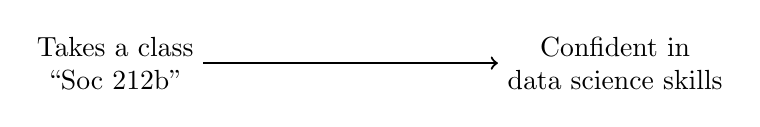
\begin{tikzpicture}[x = 2.5in, y = .5in]
\node[align = center] (a) at (0,0) {Takes a class\\``Soc 212b''};
\node[align = center] (y) at (1,0) {Confident in\\data science skills};
\draw[->, thick] (a) -- (y);
\end{tikzpicture}
\end{center}

\end{frame}

\begin{frame}{Outcome model: A visual example}

\begin{center}
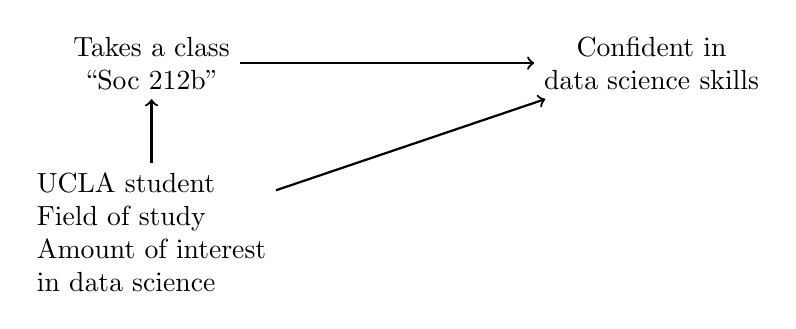
\begin{tikzpicture}[x = 2.5in, y = .5in]
\node[align = center] (a) at (0,0) {Takes a class\\``Soc 212b''};
\node[align = center] (y) at (1,0) {Confident in\\data science skills};
\draw[->, thick] (a) -- (y);
\node[anchor = north, align = left] (x) at (0,-1) {UCLA student\\Field of study\\Amount of interest\\in data science};
\draw[->, thick] (x) -- (a);
\draw[->, thick] (x) -- (y);
\end{tikzpicture}
\end{center}
Suppose these are a sufficient adjustment set.

\end{frame}

\begin{frame}{Outcome model: A visual example}

\textbf{Nonparametric estimation:}\vskip .1in
For each student in the class, find someone else who
\begin{itemize}
\item is a student at UCLA
\item shares your field of study
\item is exactly as interested in data science as you are
\item but did not take this class
\end{itemize} \vskip .1in
Use your \textbf{match} to infer your $Y_i^\text{No 212b}$ for people like you:

$$\E(Y^0\mid \vec{X} = \vec{x}_i) = \underbrace{\E(Y\mid A = 0,\vec{X} = \vec{x}_i)}_\text{estimated from your match}$$
since we have assumed conditional exchangeability given $\vec{X}$.

\end{frame}

\begin{frame}{Outcome model: A visual example}

\begin{tikzpicture}[x = \textwidth, y = .9\textheight]
\node[anchor = west] at (.75,.5) {\includegraphics{figures/legend}};
\node<1>[anchor = west] at (0,.5) {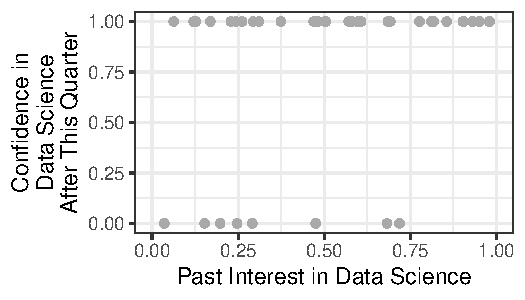
\includegraphics{figures/p1}};
\node<2>[anchor = west] at (0,.5) {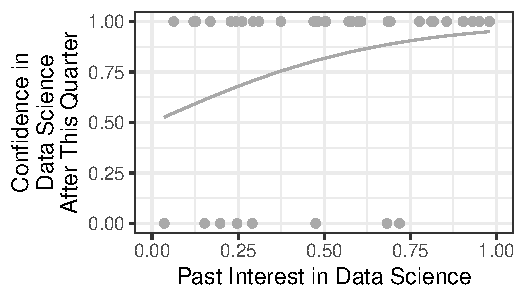
\includegraphics{figures/p2}};
\node<3>[anchor = west] at (0,.5) {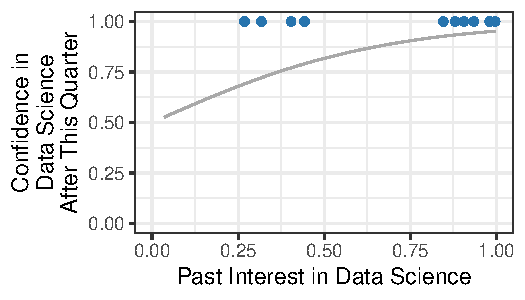
\includegraphics{figures/p3}};
\node<4>[anchor = west] at (0,.5) {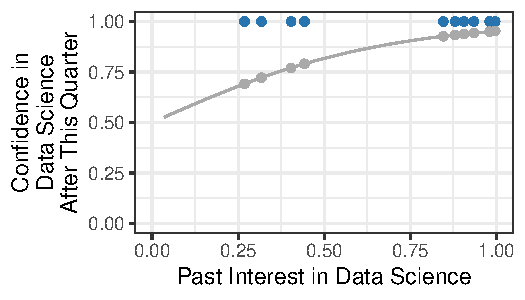
\includegraphics{figures/p4}};
\node<5>[anchor = west] at (0,.5) {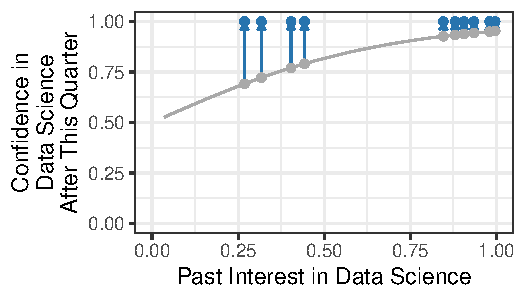
\includegraphics{figures/p5}};
\node<1>[anchor = west] at (0,.1) {1) Find control units who didn't take this class};
\node<2>[anchor = west] at (0,.1) {2) Model their outcomes given pre-treatment variables};
\node<3>[anchor = west] at (0,.1) {3) Find the treated units of interest};
\node<4>[anchor = west] at (0,.1) {4) Predict their counterfactual outcomes};
\node<5>[anchor = west] at (0,.1) {5) Infer causal effect for each person. Average over people};
\end{tikzpicture}

\end{frame}

\begin{frame}{Outcome model: A visual example}

\begin{tikzpicture}[x = \textwidth, y = .9\textheight]
%\node[anchor = west] at (.75,.9) {\includegraphics{legend}};
\node[anchor = west] at (.75,.9) {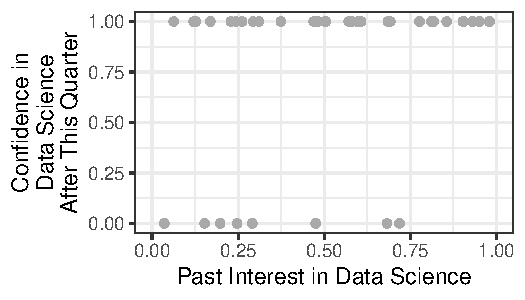
\includegraphics[scale = .3]{figures/p1}};
\node[anchor = west] at (.75,.7) {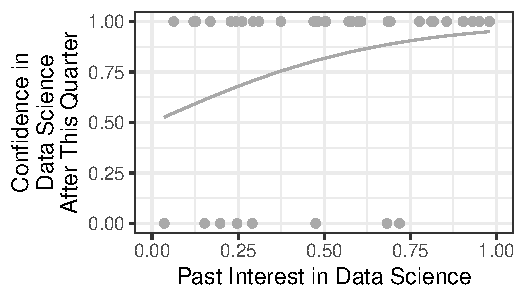
\includegraphics[scale = .3]{figures/p2}};
\node[anchor = west] at (.75,.5) {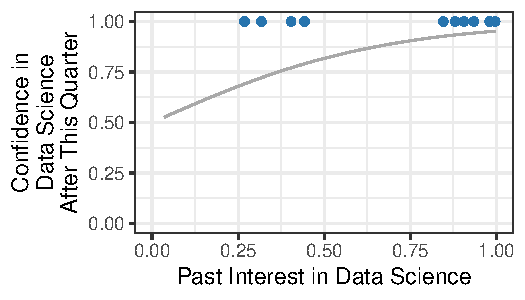
\includegraphics[scale = .3]{figures/p3}};
\node[anchor = west] at (.75,.3) {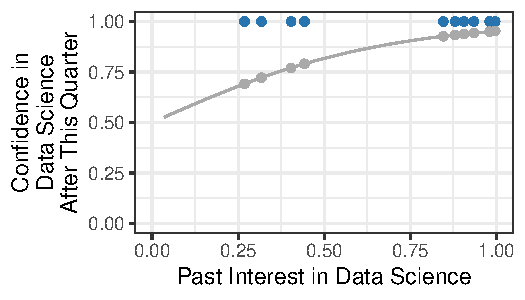
\includegraphics[scale = .3]{figures/p4}};
\node[anchor = west] at (.75,.1) {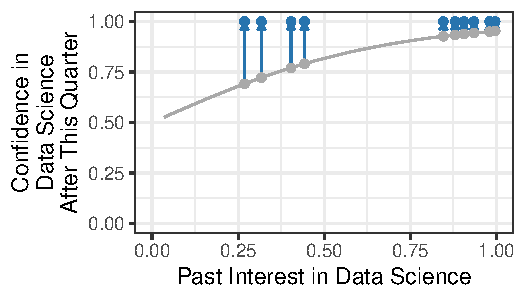
\includegraphics[scale = .3]{figures/p5}};
\node[anchor = west, scale = .8] at (0,.9) {1) Find control units who didn't take this class};
\node[anchor = west, scale = .8] at (0,.7) {2) Model their outcomes given pre-treatment variables};
\node[anchor = west, scale = .8] at (0,.5) {3) Find the treated units of interest};
\node[anchor = west, scale = .8] at (0,.3) {4) Predict their counterfactual outcomes};
\node[anchor = west, scale = .8] at (0,.1) {5) Infer causal effect for each person. Average over people};
\end{tikzpicture}

\end{frame}

\begin{frame}{Outcome model: A visual example}


\begin{tikzpicture}[x = \textwidth, y = .8\textheight]
\node at (0,0) {};
\node at (1,1) {};
\foreach \i in {.3, .4, .5,.6,.7,.8} {
	\draw[fill = blue, opacity = .3, color = blue] (.05,\i) rectangle (.25,\i + .1) {};
	\draw[fill = seagreen, opacity = .3, color = seagreen] (.25,\i) rectangle (.45,\i + .1) {};
}
\node[font = \footnotesize] at (.15,.85) {$Y_1^\text{Takes 212b}$};
\node[font = \footnotesize] at (.15,.75) {$Y_2^\text{Takes 212b}$};
\node[font = \footnotesize] at (.15,.55) {$Y_4^\text{Takes 212b}$};
\node[font = \footnotesize] at (.15,.65) {$Y_3^\text{Takes 212b}$};
\node[font = \footnotesize] at (.15,.45) {$Y_5^\text{Takes 212b}$};
\node[font = \footnotesize] at (.15,.35) {$Y_6^\text{Takes 212b}$};
\only<1>{
\node[font = \footnotesize] at (.35,.85) {?};
\node[font = \footnotesize] at (.35,.75) {?};
\node[font = \footnotesize] at (.35,.55) {?};
\node[font = \footnotesize] at (.35,.65) {?};
\node[font = \footnotesize] at (.35,.45) {?};
\node[font = \footnotesize] at (.35,.35) {?};
}
\only<2->{
\node[font = \footnotesize] at (.35,.85) {$\hat{Y}_1^\text{No 212b}$};
\node[font = \footnotesize] at (.35,.75) {$\hat{Y}_2^\text{No 212b}$};
\node[font = \footnotesize] at (.35,.55) {$\hat{Y}_4^\text{No 212b}$};
\node[font = \footnotesize] at (.35,.65) {$\hat{Y}_3^\text{No 212b}$};
\node[font = \footnotesize] at (.35,.45) {$\hat{Y}_5^\text{No 212b}$};
\node[font = \footnotesize] at (.35,.35) {$\hat{Y}_6^\text{No 212b}$};
}
\node[anchor = north, align = center, font = \footnotesize, blue] at (.15, .3) {Outcome\\under\\212b};
\node[anchor = north, align = center, font = \footnotesize, seagreen] at (.35, .3) {Outcome\\under\\no 212b};
\node[anchor = south, rotate = 90, align = center] at (.05, .6) {Each Row is a\\Student in This Class};
\node<3->[anchor = north west] at (.52,.9) {\textbf{General approach}};
\node<4->[anchor = north west] at (.52,.8) {1) Define potential outcomes};
\node<5->[anchor = north west] at (.52,.72) {2) Define target population};
\node<6->[anchor = north west] at (.52,.64) {3) Make causal assumptions};
\node<7->[anchor = north west] at (.52,.56) {4) Model unobserved outcomes};
\node<8->[anchor = north west] at (.52,.48) {5) Predict them};
\node<9->[anchor = north west] at (.52,.4) {6) Report an average};
\end{tikzpicture}

\end{frame}

\section{Coding Example}

\begin{frame}{Outcome model: A coding example}

Since this part is code, it will follow the website instead of slides.

\end{frame}

\section{With ML}

\begin{frame}
\huge Predicting outcomes for causal inference with machine learning
\end{frame}

\begin{frame}{Outcome model: You are now an expert}

\begin{enumerate}
\item Assume a DAG
\begin{center}
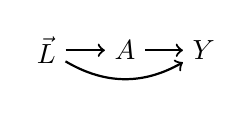
\begin{tikzpicture}
\node (l) at (-1,0) {$\vec{L}$};
\node (a) at (0,0) {$A$};
\node (y) at (1,0) {$Y$};
\draw[->, thick] (l) -- (a);
\draw[->, thick] (l) to[bend right] (y);
\draw[->, thick] (a) -- (y);
\end{tikzpicture}
\end{center}
\item By consistency, exchangeability, and positivity, $$\underbrace{\E(Y^a\mid\vec{L} = \vec\ell)}_{\text{Causal}} = \underbrace{\E(Y\mid A = a, \vec{L} = \vec\ell)}_{\text{Statistical}}$$
\item Using regression, estimate $\hat\E(Y\mid A, \vec{L})$
\item Predict unknown potential outcomes and average
$$\hat\E(Y^a) = \frac{1}{n}\sum_{i=1}^n \hat\E\left(Y\mid A = a, \vec{L} = \vec\ell_i\right)$$
\end{enumerate}
\bblue{Big idea:} Why constrain ourselves to regression for $\hat\E(Y\mid A, \vec{L})$?

\end{frame}

\begin{frame}

Hill, Jennifer L. 2011.\\``\bref{https://doi.org/10.1198/jcgs.2010.08162}{Bayesian nonparametric modeling for causal inference.}"\\Journal of Computational and Graphical Statistics 20.1:217-240. \vskip .1in
\begin{itemize}
\item Binary treatment \hfill (simulated)
\item Continuous confounder $X$ \hfill (simulated)
\end{itemize} \vskip .1in
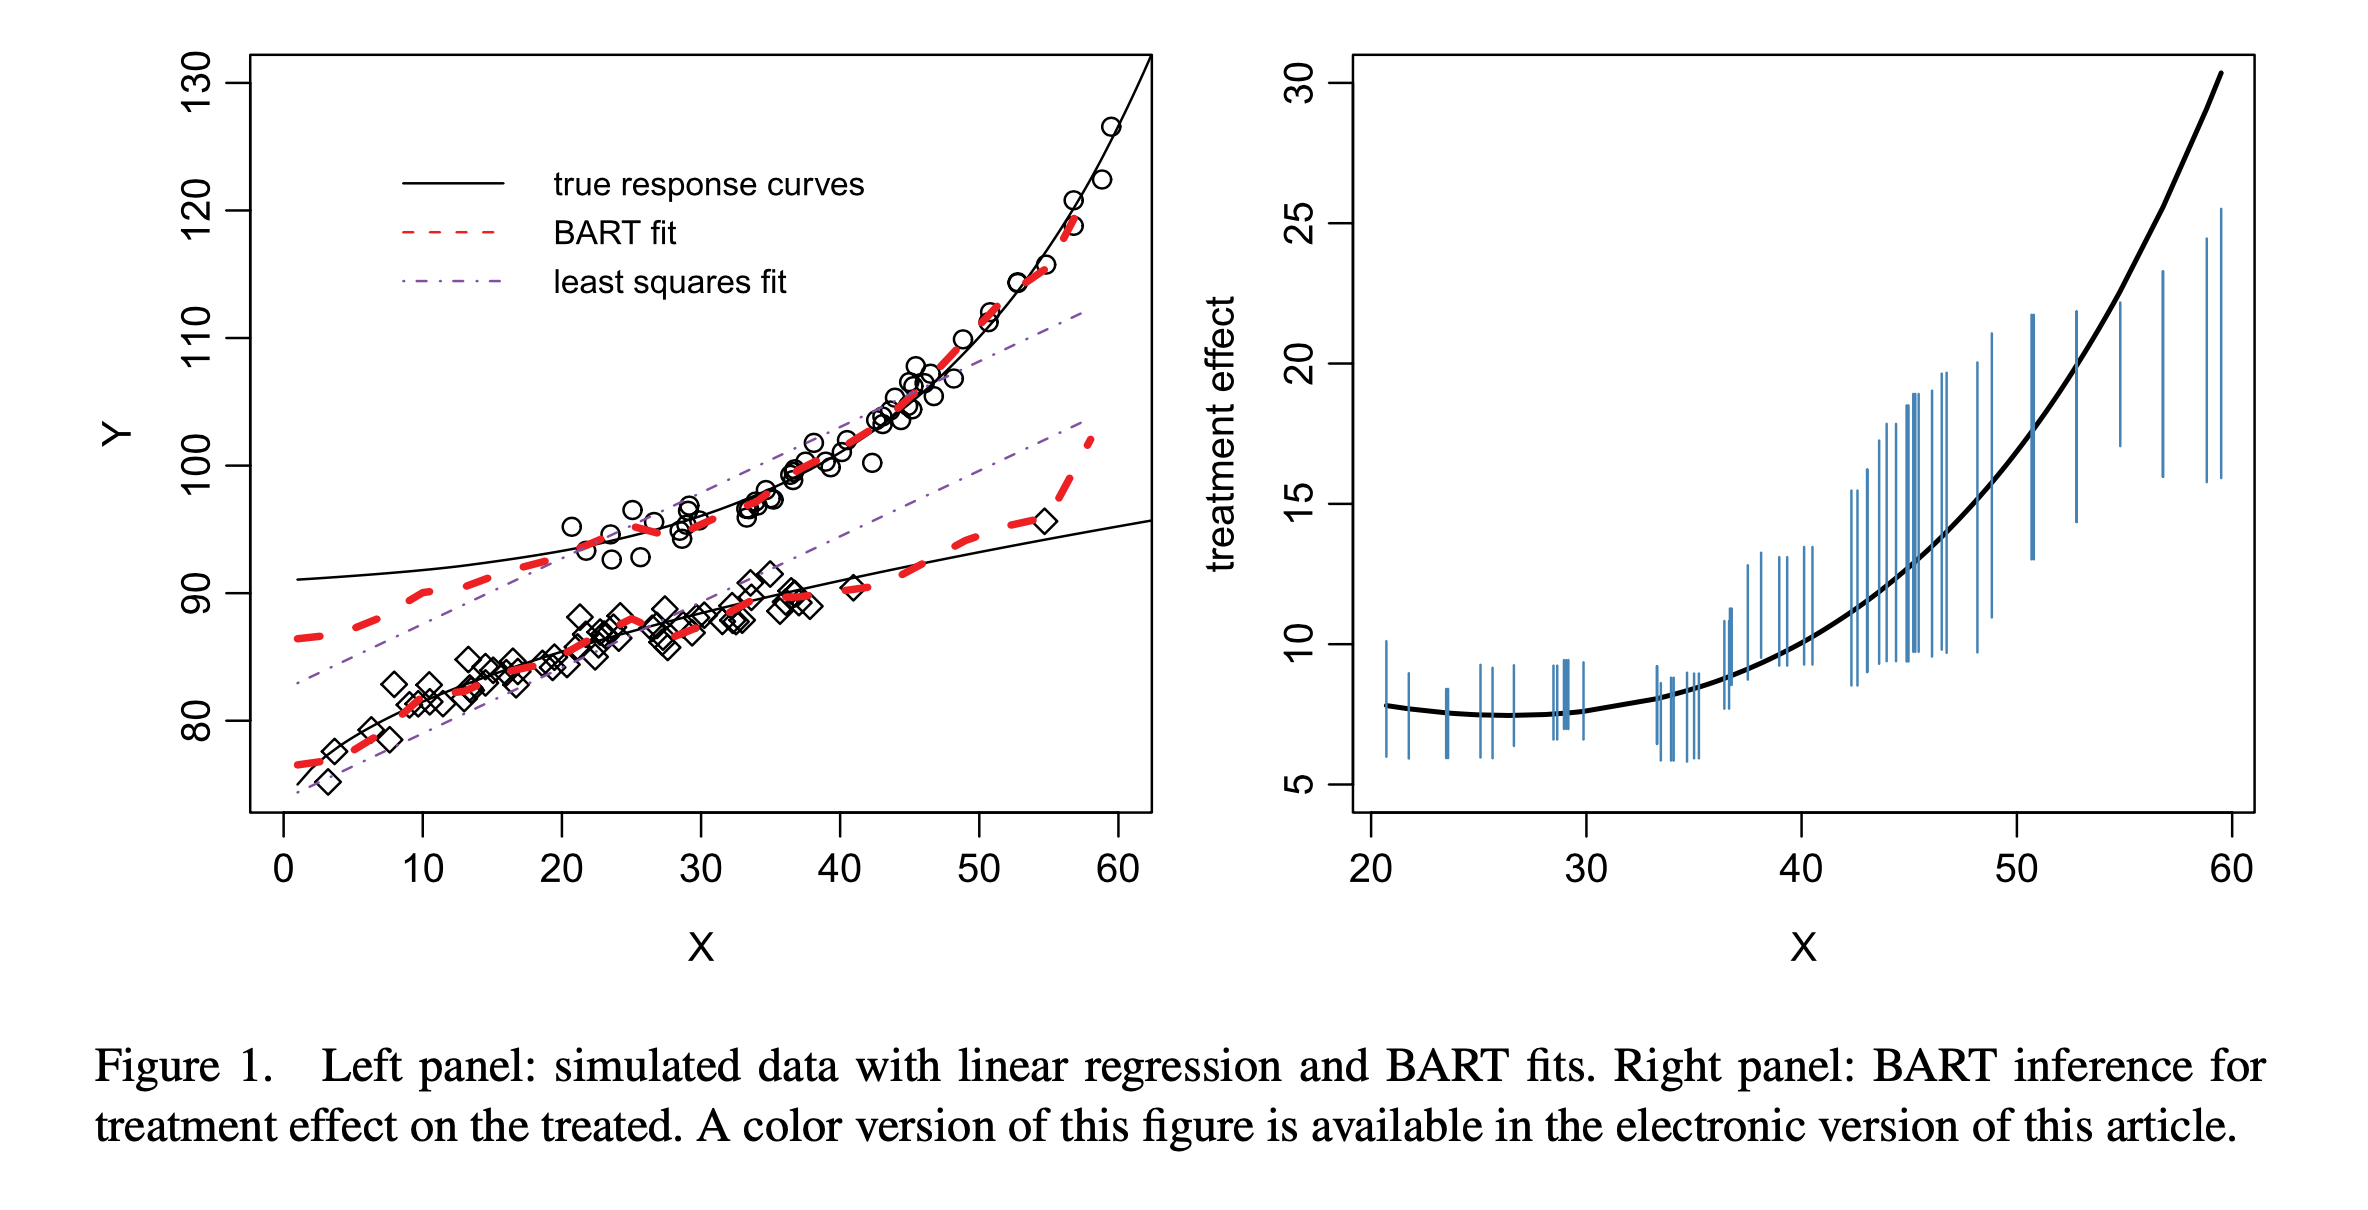
\includegraphics[width = \textwidth]{figures/hill2011_fig1}

\end{frame}

\begin{frame}[t]{How did she do that?\footnote{Chipman, Hugh A., Edward I. George, and Robert E. McCulloch. ``\bref{https://projecteuclid.org/journals/annals-of-applied-statistics/volume-4/issue-1/BART-Bayesian-additive-regression-trees/10.1214/09-AOAS285.full}{BART: Bayesian additive regression trees.}" The Annals of Applied Statistics 4.1 (2010): 266-298.}}
\vskip .2in
1) Learn an automated partitioning of the data (aka a ``tree'')
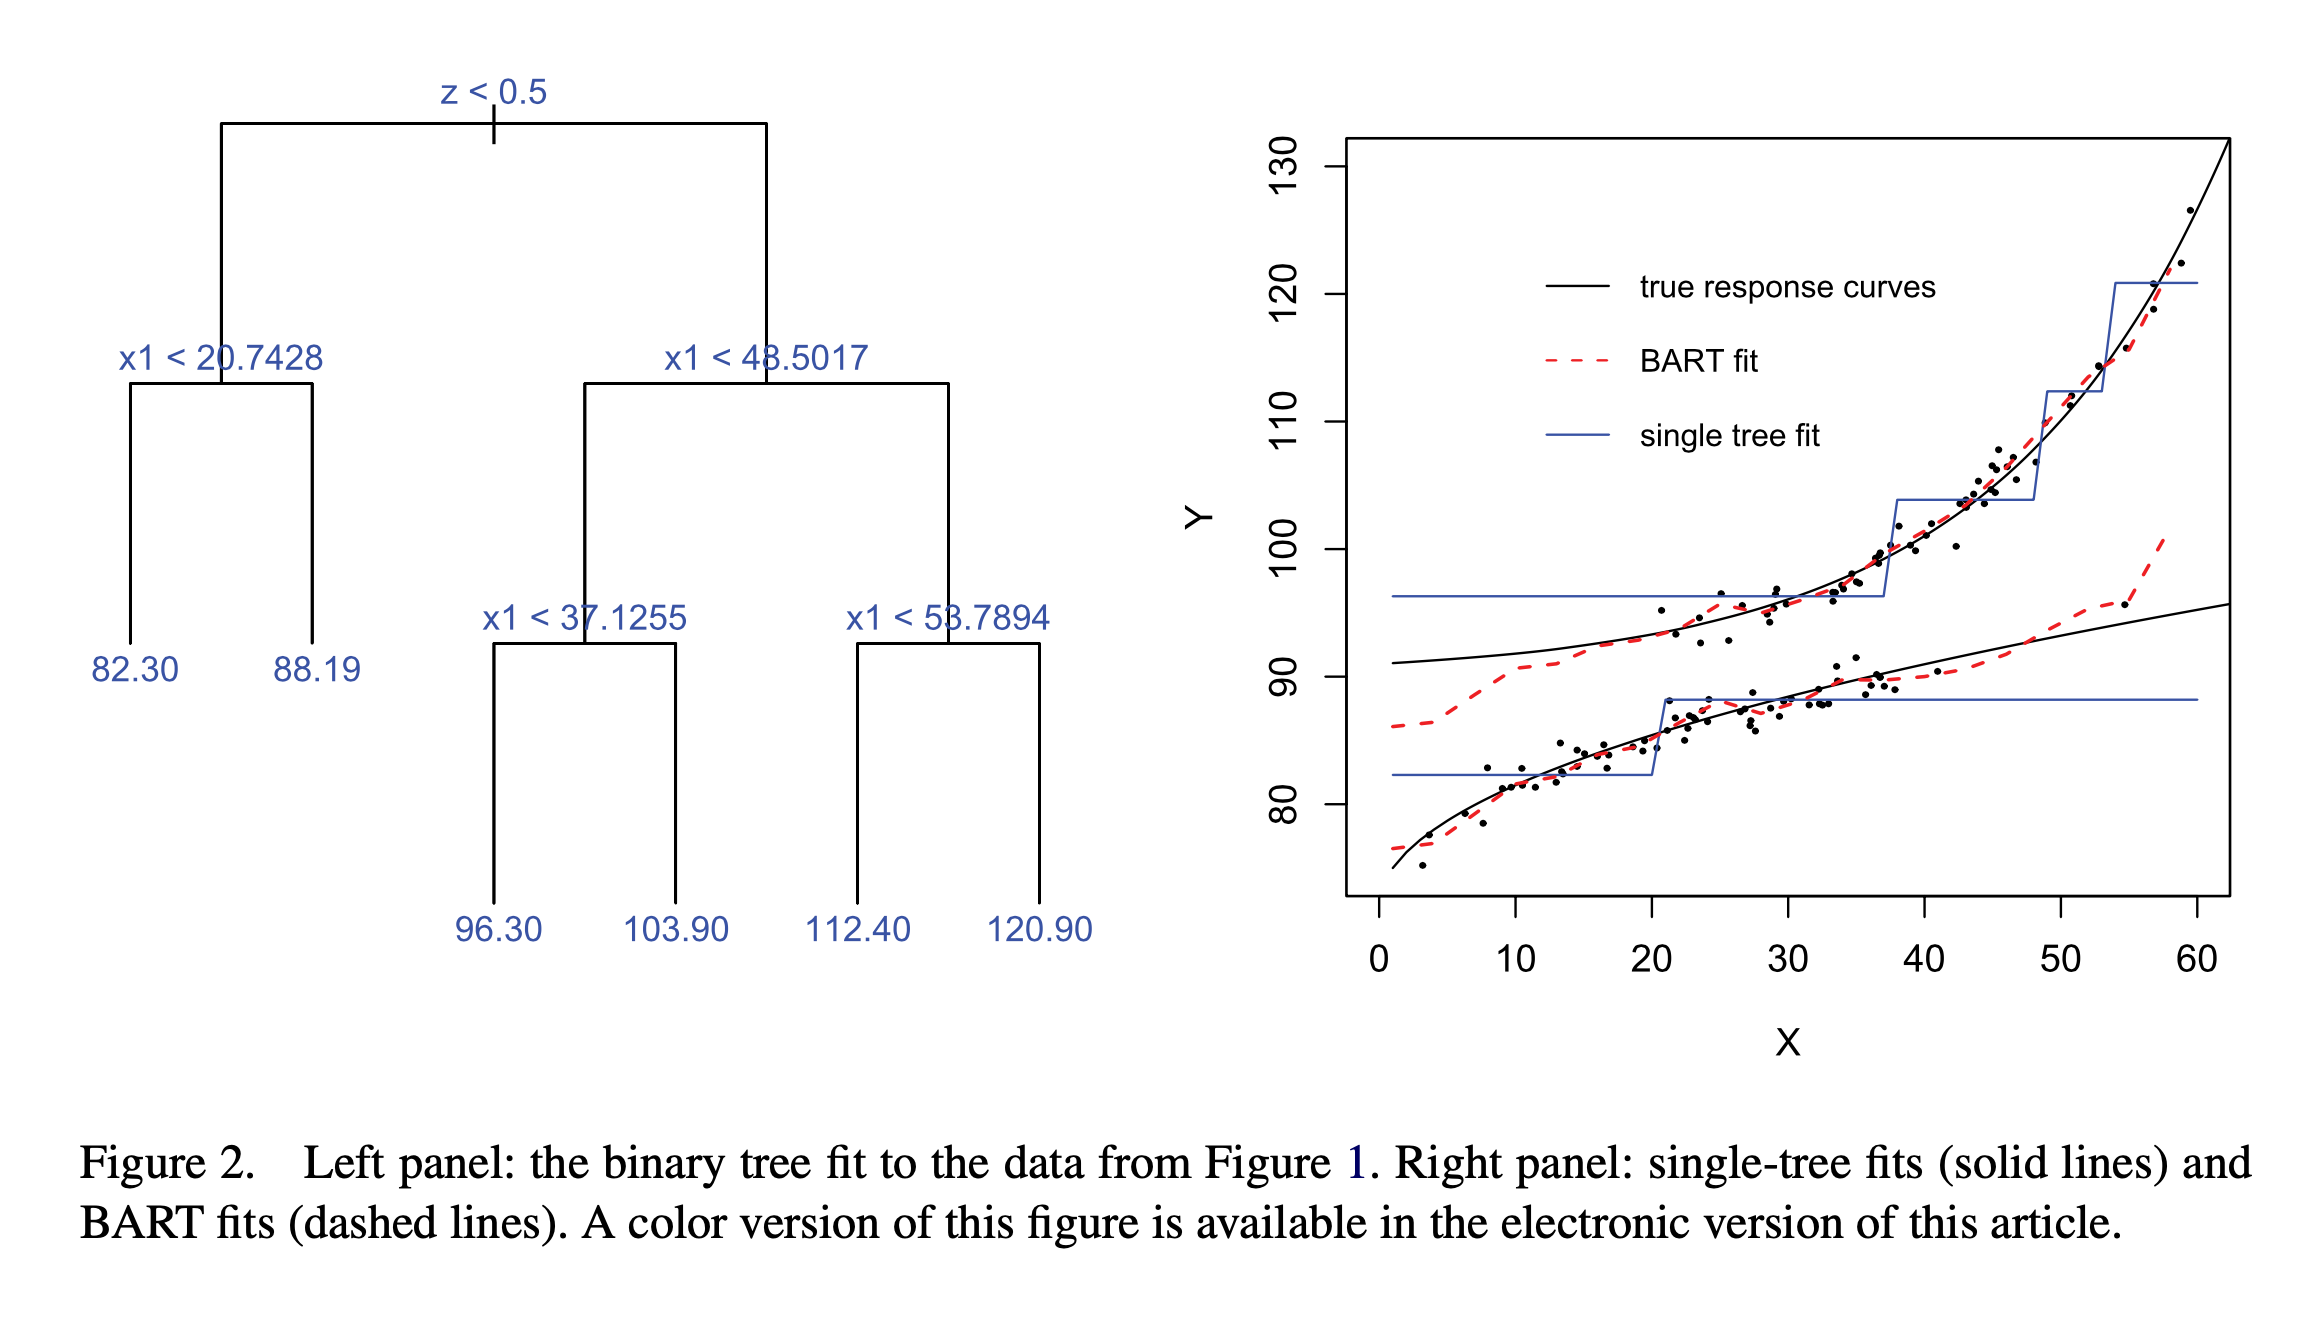
\includegraphics[width = \textwidth]{figures/hill2011_fig2}
\end{frame}

\begin{frame}[t]{How did she do that?}
\vskip .2in
2) Repeat many times. Take the average.\\
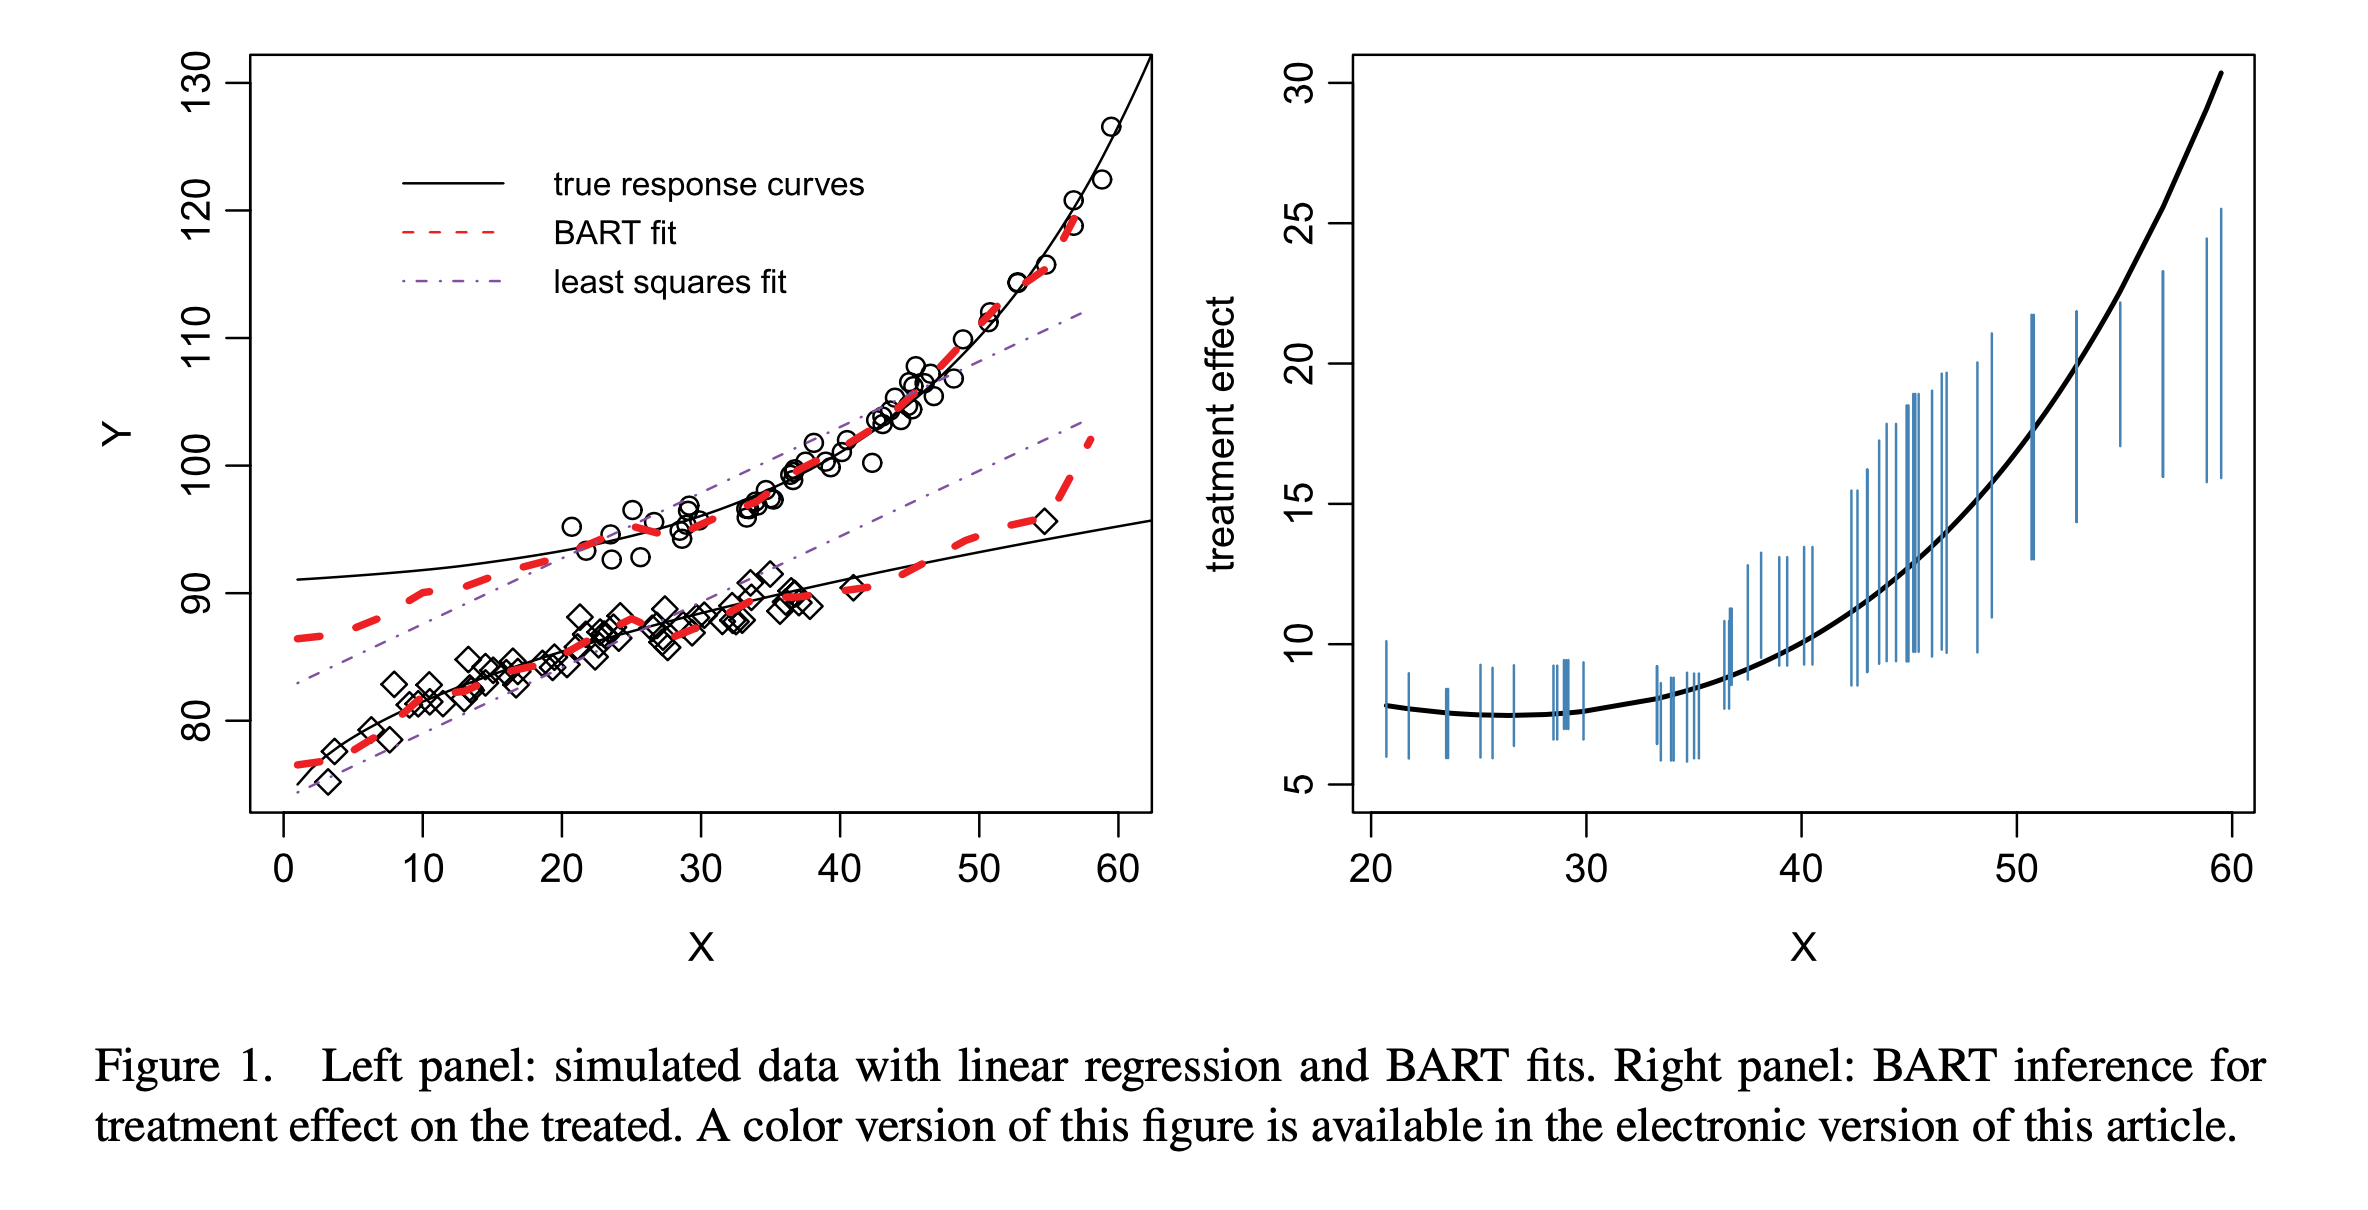
\includegraphics[width = \textwidth]{figures/hill2011_fig1}
\end{frame}

\begin{frame}{Core idea: Causal assumptions unlock machine learning\footnote{Caveat: There are ways to do even better. This is just a start.\\See Van der Laan, M. J., \& Rose, S. (2018). \bref{https://link.springer.com/content/pdf/10.1007/978-3-319-65304-4.pdf}{Targeted learning in data science.} Springer International Publishing.}}
Once you make this assumption
\begin{center}
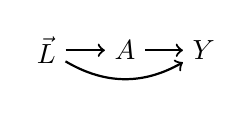
\begin{tikzpicture}
\node (l) at (-1,0) {$\vec{L}$};
\node (a) at (0,0) {$A$};
\node (y) at (1,0) {$Y$};
\draw[->, thick] (l) -- (a);
\draw[->, thick] (l) to[bend right] (y);
\draw[->, thick] (a) -- (y);
\end{tikzpicture}
\end{center}
you get to do this
\begin{center}
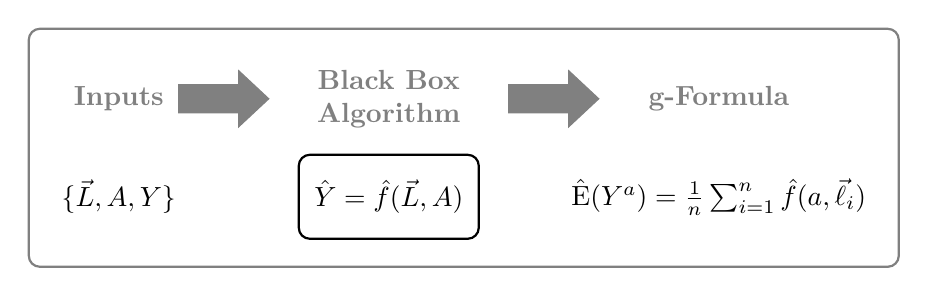
\begin{tikzpicture}[x = 1.5in, y = .7in]
\node[gray, font = \bf] at (-1,.7) {Inputs};
\node[align = center, gray, font = \bf] at (-.1,.7) {Black Box\\Algorithm};
\node[gray, font = \bf] at (1,.7) {g-Formula};
\node at (-1,0) {$\{\vec{L},A,Y\}$};
\node at (-.1,0) {$\hat{Y} = \hat{f}(\vec{L},A)$};
\node at (1,0) {$\hat\E(Y^a) = \frac{1}{n}\sum_{i=1}^n \hat{f}(a,\vec\ell_i)$};
\draw[thick, rounded corners] (-.4,-.3) rectangle (.2,.3);
\draw[thick, gray, rounded corners] (-1.3,-.5) rectangle (1.6, 1.2);
\draw[draw = gray, fill = gray] (-.8,.8) -- (-.8,.6) -- (-.6,.6) -- (-.6,.5) -- (-.5,.7) -- (-.6,.9) -- (-.6,.8) -- cycle;
\draw[draw = gray, fill = gray] (.3,.8) -- (.3,.6) -- (.5,.6) -- (.5,.5) -- (.6,.7) -- (.5,.9) -- (.5,.8) -- cycle;
\end{tikzpicture}
\end{center}
\end{frame}

\begin{frame}
There are \bblue{so many} algorithms you might use!
\end{frame}

\begin{frame}
\centering
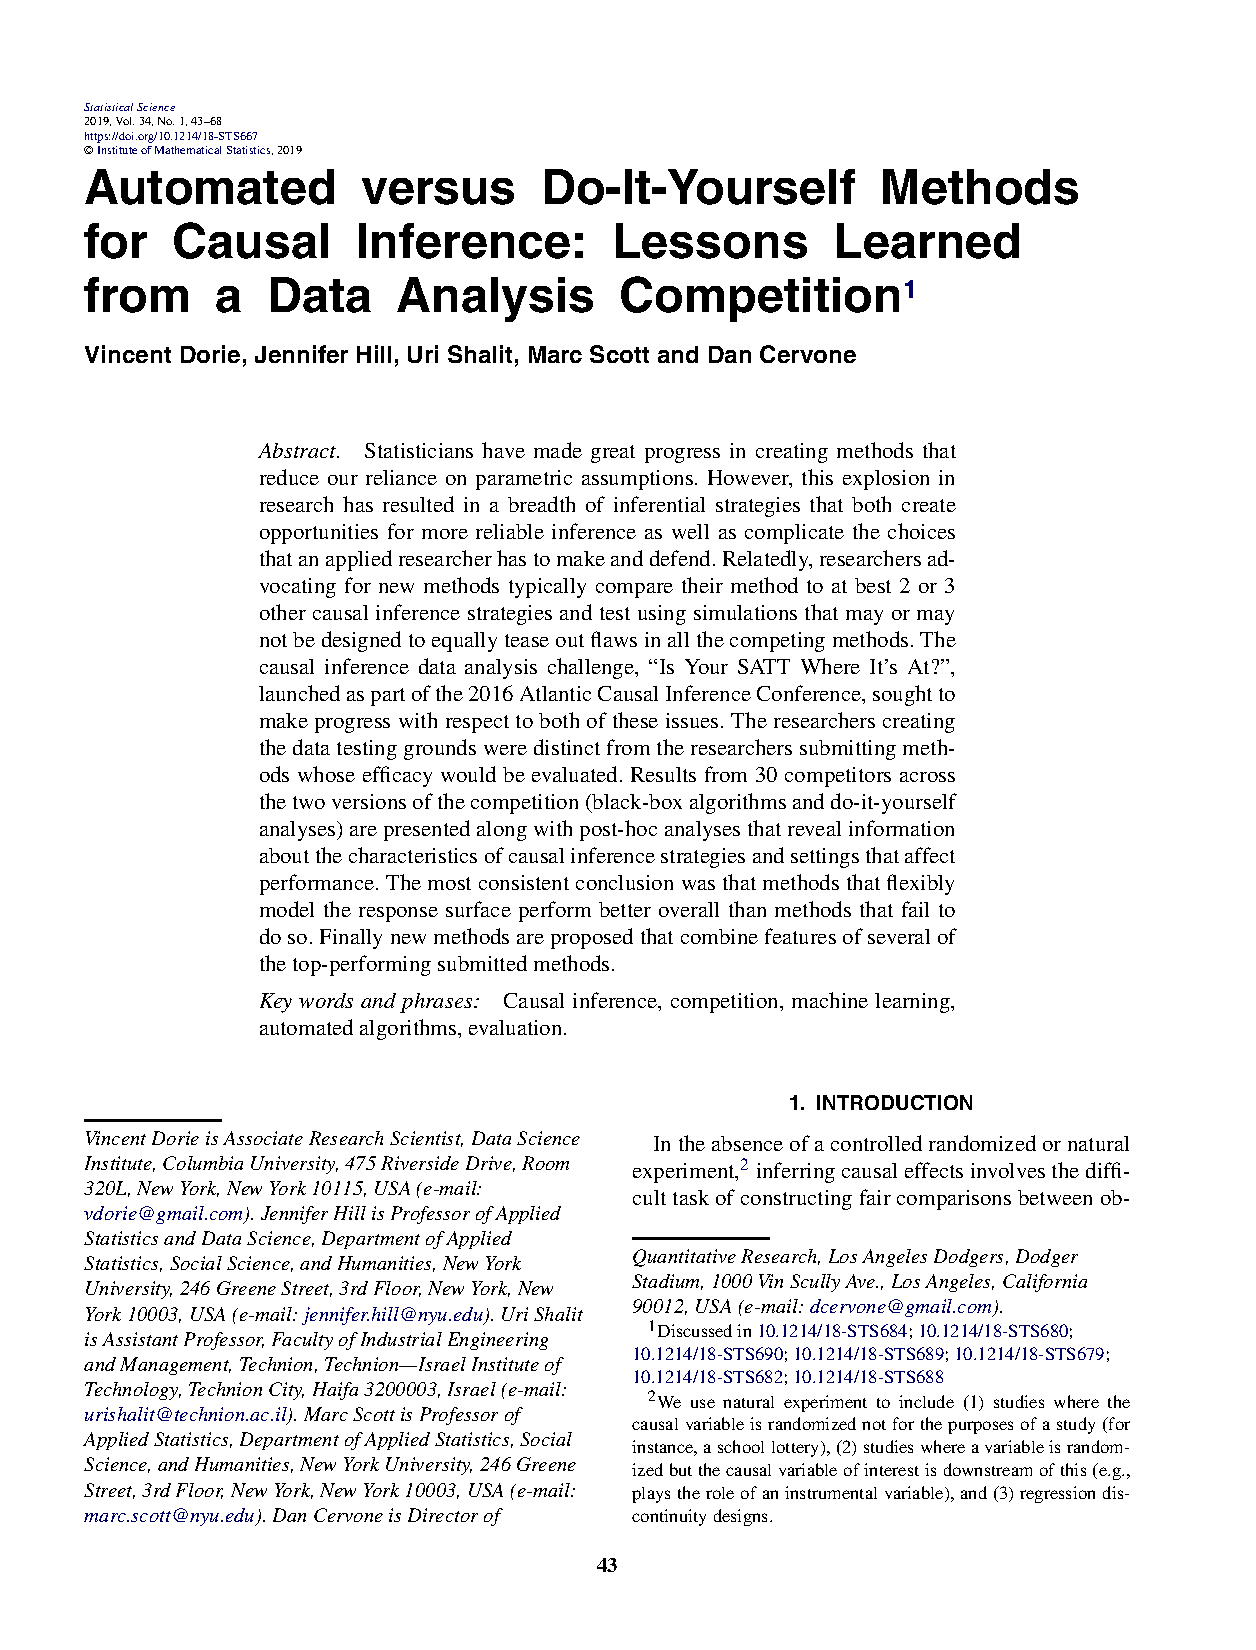
\includegraphics[height = \textheight]{figures/dorie_p1}
\end{frame}

\begin{frame}{Dorie et al. 2019\footnote{
Dorie, V., Hill, J., Shalit, U., Scott, M., \& Cervone, D. (2019).\\
``\bref{https://projecteuclid.org/journals/statistical-science/volume-34/issue-1/Automated-versus-Do-It-Yourself-Methods-for-Causal-Inference/10.1214/18-STS667.full}{Automated versus do-it-yourself methods for causal inference: Lessons learned from a data analysis competition.}'' Statistical Science, 34(1), 43-68. See also \blue{\url{https://jenniferhill7.wixsite.com/acic-2016/competition}}}: Is Your SATT Where It's At?}

\begin{itemize} \pause
\item Goal: The Sample Average Treatment Effect on the Treated
$$\text{SATT} = \frac{1}{n_\text{Treated}}\sum_{i:A_i = 1} \left(Y_i^1 - Y_i^0\right)$$ \pause
\item Simulated data. SATT was known to organizers \pause
\item Confounders were defined by the organizers \pause
\item Participants could use any algorithm to estimate SATT \pause
\item 30 teams attempted the task
\end{itemize}

\end{frame}

\section{Warnings}

\begin{frame}
\huge{Words of Warning}
\end{frame}

\begin{frame}{Good prediction of $Y$ does not guarantee\\good estimation of $Y^1-Y^0$} \pause

\begin{itemize}
\item there may be unmeasured confounding
\item the regularization in machine learning models can induce a large bias
\item to predict $Y^1$, the model is trained on treated units. But untreated units may have a very different distribution of $\vec{X}$
\end{itemize}

\end{frame}

\begin{frame}{Good prediction of $Y$ does not guarantee\\good estimation of $Y^1-Y^0$: An example}

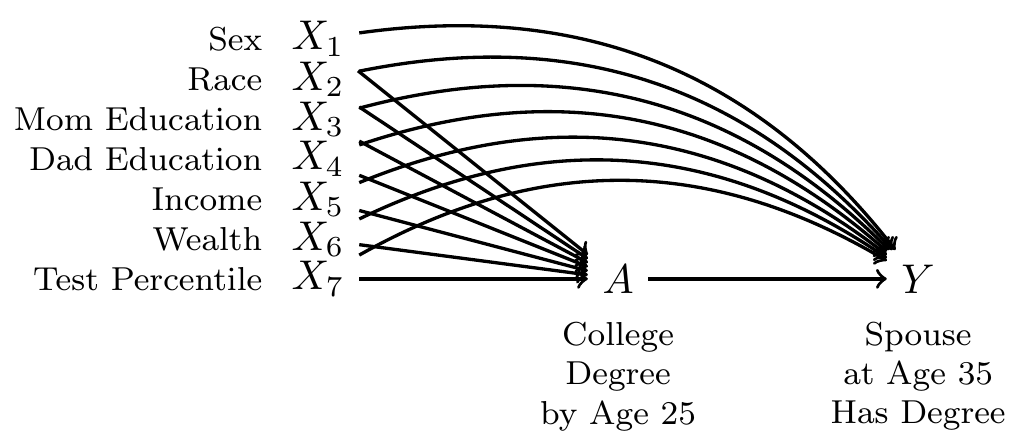
\includegraphics[width = .4\textwidth]{figures/dag_example}
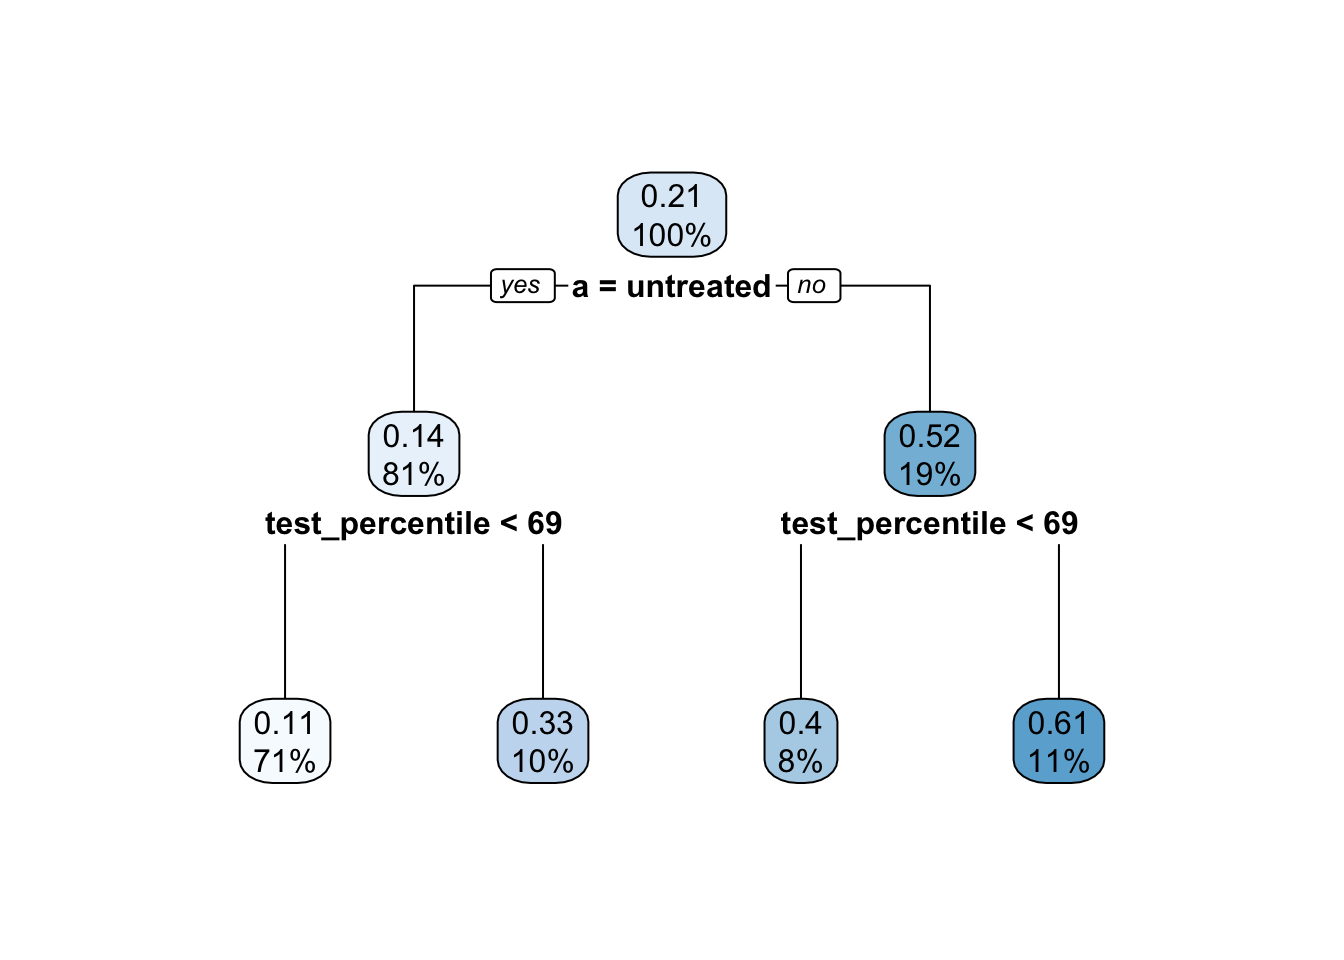
\includegraphics[width = .58\textwidth]{figures/tree_example}\\
What is troubling about this tree, if used for causal inference?

\end{frame}

\goalsframe

\end{document}
